% BEGIN PREAMBEL
\documentclass[9pt, xcolor=dvipsnames]{beamer}
\usepackage[british]{babel}
\usepackage{multimedia}
\usepackage{amsmath,amsfonts,amssymb}
\usepackage{upgreek}
\usepackage{pgfpages}
\usepackage[version=3]{mhchem}
\usepackage{lmodern}
\usepackage{graphicx}
\usepackage{multicol}
\usepackage{color}
\usepackage{xcolor,fontawesome}
\usepackage{wrapfig}
\usepackage{siunitx}
\usepackage{fontspec}
\usepackage{tikz}
\usepackage{textpos}
\usepackage{booktabs}
\usepackage{caption}
\usepackage{subcaption}
\usepackage{wasysym}
\usepackage{animate}
\usepackage{tabularx}
\usepackage{ETHlogo}
\usepackage{animate}
\usepackage{todonotes}
\newfontfamily\ubuntu{Ubuntu}
\newcommand{\as}{\\[14pt]}
\newcommand{\s}{\\[7pt]}
\newcommand{\is}{\\[2pt]}
\newcommand{\no}{\noindent}
\newcommand{\ka}{\hspace*{0.5cm}}
\newcommand{\ma}{\hspace*{1cm}}
\newcommand{\ga}{\hspace*{1.5cm}}
\newcommand{\li}{\left|}
\newcommand{\re}{\right|}
\newcommand{\const}{\text{const.}}
\newcommand{\z}{\text}
\newcommand{\terminal}[1]{\colorbox{black}{\textcolor{white}{{\fontfamily{phv}\selectfont \scriptsize{#1}}}}}
\newcommand{\plugin}[1]{\textit{\flq#1\frq}}
\newcommand{\ra}{$\rightarrow$ }
\definecolor{cadmiumgreen}{rgb}{0.0, 0.42, 0.24}
\newcommand{\itemfill}{\setlength{\itemsep}{\fill}}
\newcommand{\orderof}[1]{$\mathcal{O}\left(#1\right)$}
\newcommand{\fig}[2]{\begin{figure}\centering\includegraphics[height={#2}\textheight]{#1}\end{figure}}
\newcommand{\figc}[3]{\begin{figure}\centering\includegraphics[height={#2}\textheight]{#1}\caption{#3}\end{figure}}
\newcommand{\figp}[2]{\begin{figure}\centering\includegraphics[width={#2}\textheight, angle=-90]{#1}\end{figure}}
\newcommand{\subfig}[4][0.45]{\begin{subfigure}{{#1}\textwidth}\centering
			\includegraphics[height={#3}\textheight]{#2}
			\caption{#4}\end{subfigure}}
\newcommand{\subfiga}[3][0.45]{\begin{subfigure}{{#1}\textwidth}\centering\includegraphics[height={#3}\textheight]{#2}\end{subfigure}}
\newcommand{\subfigp}[3]{\begin{subfigure}{0.45\textwidth}\centering\includegraphics[width={#2}\textheight, angle=-90]{#1}
			\caption{#3}\end{subfigure}}
\newcommand{\subfigpa}[3][0.45]{\begin{subfigure}{#1\textwidth}\centering\includegraphics[width={#3}\textheight, angle=-90]{#2}\end{subfigure}}
\newcommand{\ttb}{$\z{t}\overline{\z{t}}$}

\usetheme{Boadilla}
\graphicspath{ {Pics/} }
\makeatletter
\def\input@path{ {sections/} }
\makeatother
\usecolortheme[named=ForestGreen]{structure}
\useoutertheme{miniframes}
\beamertemplatenavigationsymbolsempty
\makeindex
\author[M. Reichmann]{Michael Reichmann}
\institute[\textbf{\textit{ETH}}\scalebox{.6}{\textit{Z\"{u}rich}}]{Swiss Federal Institute of Technology Zurich}
\AtBeginSection{\frame[noframenumbering]{\sectionpage}}

\setbeamercolor{frametitle}{bg=date in head/foot.bg!20!white}

%% TITLE PAGE
\defbeamertemplate*{title page}{customized}[1][] {
	\ETHlogo[3cm]
	\vspace*{-33pt}
	\begin{figure}[t]
		\flushright
		
\includegraphics[height=.9cm]{IPP}
	\end{figure}
	\vspace*{-10pt}
	\begin{figure}
		\centering
		\includegraphics[width=.4\textheight, angle=-90]{\inserttitlegraphic}
	\end{figure}
	\begin{block}{}
		\centering
		\vspace*{1pt}
		\usebeamerfont{title}\usebeamercolor[fg]{title}\textbf{\inserttitle}\\\vspace*{5pt}
		\usebeamerfont{subtitle}\insertsubtitle\\\vspace*{1pt}
	\end{block}
	\vspace*{10pt}
	\centering
	\color{black}
	\usebeamerfont{author}\textbf{\insertauthor}\par\vspace*{5pt}
	\usebeamerfont{date}\insertdate\par
}

%% FOOTLINE
\setbeamertemplate{footline}
{
  \leavevmode%
  \hbox{%
  \begin{beamercolorbox}[wd=.3\paperwidth,ht=2.25ex,dp=1ex,center]{author in head/foot}%
    \usebeamerfont{author in head/foot}\insertshortauthor\hspace*{2pt}
    (
\includegraphics[height=3.5pt]{ETHLogoWhite})
  \end{beamercolorbox}%
  \begin{beamercolorbox}[wd=.4\paperwidth,ht=2.25ex,dp=1ex,center]{title in head/foot}%
    \usebeamerfont{title in head/foot}\insertshorttitle
  \end{beamercolorbox}%
  \begin{beamercolorbox}[wd=.3\paperwidth,ht=2.25ex,dp=1ex,right]{date in head/foot}%
    \usebeamerfont{date in head/foot}\insertdate\hspace*{3em}
    \insertframenumber{} / \inserttotalframenumber\hspace*{1ex}
  \end{beamercolorbox}}%
  \vskip0pt%
}
 
%% SECTION PAGE
\setbeamertemplate{section page}
{
    \begin{centering}
		\usebeamerfont{title}Section \insertsectionnumber\\\vspace*{.7cm}
		\begin{beamerboxesrounded}[shadow=true, lower=frametitle]{}
			\centering
			\vspace*{3pt}
			\usebeamerfont{frametitle}\textbf{\insertsection}\par
			\vspace*{3pt}
		\end{beamerboxesrounded}
    \end{centering}
}

\title[Diamond Pad Detectors]{Signal Behaviour of pCVD Diamond Pad Detectors Depending on Incident Particle Flux}
\subtitle{ADAMAS Workshop}
\titlegraphic{PadFull1}
\date{27th November 2017}
% END PREAMBEL

\begin{document}

% ============= TITLE PAGE =============
\usebackgroundtemplate{\tikz\node[opacity=0.2] {\hspace*{-5pt}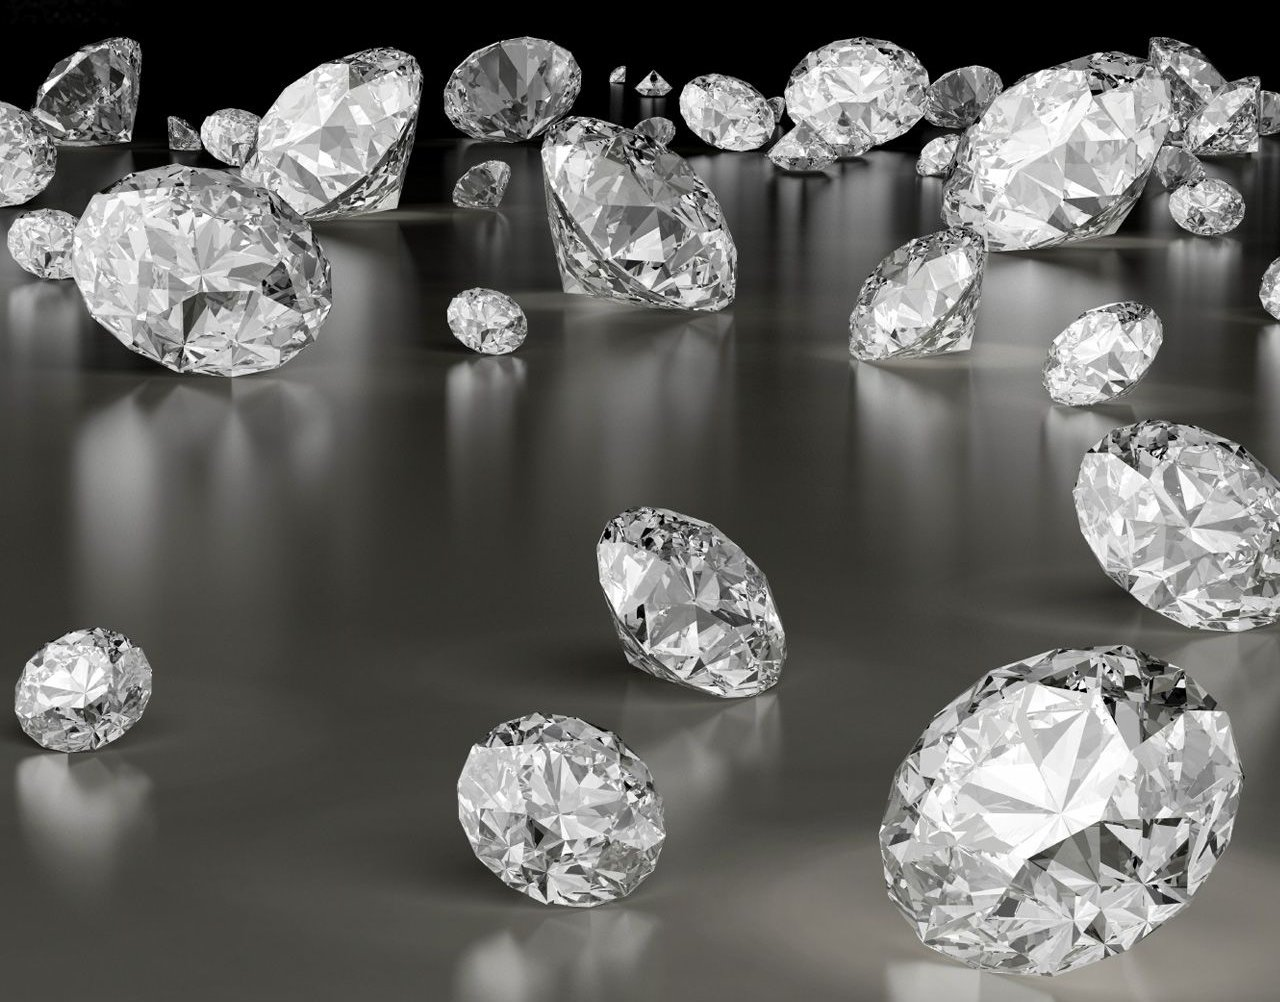
\includegraphics[height=\paperheight,width=1.05\paperwidth]{bkg.jpg}};}
\maketitle
\usebackgroundtemplate{}

% ============= TABLE OF CONTENTS ======
\begin{frame}%[allowframebreaks]
	\frametitle{Table of contents}
	\tableofcontents[hideallsubsections]   % [pausesections]
\end{frame}

% ============= 1 =============
\section{Motivation}
\begin{frame}{Motivation}

	\begin{itemize}
		\item innermost layers \ra highest radiation damage
		\item current detector is designed to survive \SI{\sim12}{month} in High-Luminosity LHC
		\item completely new regime of particle flux \orderof{\SI{}{\giga\hertz\per\centi\meter^2}}
		\item \usebeamercolor[fg]{title} \textbf{\ra R/D for more radiation tolerant detector designs and/or materials}
	\end{itemize}\vspace*{10pt}
	
	\uncover<2->{
		\textbf{\underline{Diamond as Detector Material:}}\vspace*{5pt}
		\begin{itemize}
			\itemfill
			\item advantageous properties 
			\begin{itemize}
				\itemfill
				\item radiation tolerant
				\item isolating material
				\item high charge carrier mobility
			\end{itemize}
		\end{itemize}}
	
	\uncover<3->{
		\begin{itemize}
			\item investigation of the rate effect in various detector designs:\vspace*{5pt}
			\begin{itemize} \itemfill
				\item {\usebeamercolor[fg]{title}\textbf{pad \ra full diamond as single cell readout of the whole signal \ra shown here}}
				\item pixel \ra diamond sensors on state-of-the-art pixel chips
				\item 3D \ra pixel detector with clever design to reduce drift distance
			\end{itemize}

		\end{itemize}}
		
\end{frame}

% ============= 2 =============
\section{Test Site \& Setup}
%%%%%%%%%%%%%%%%%%%%%%%% FRAME 0 %%%%%%%%%%%%%%%%%%%%%%%%%%%%%%%
\begin{frame}{Test Site}[plain]

	\begin{tikzpicture}[remember picture,overlay]
		\node[at=(current page.center)] {
			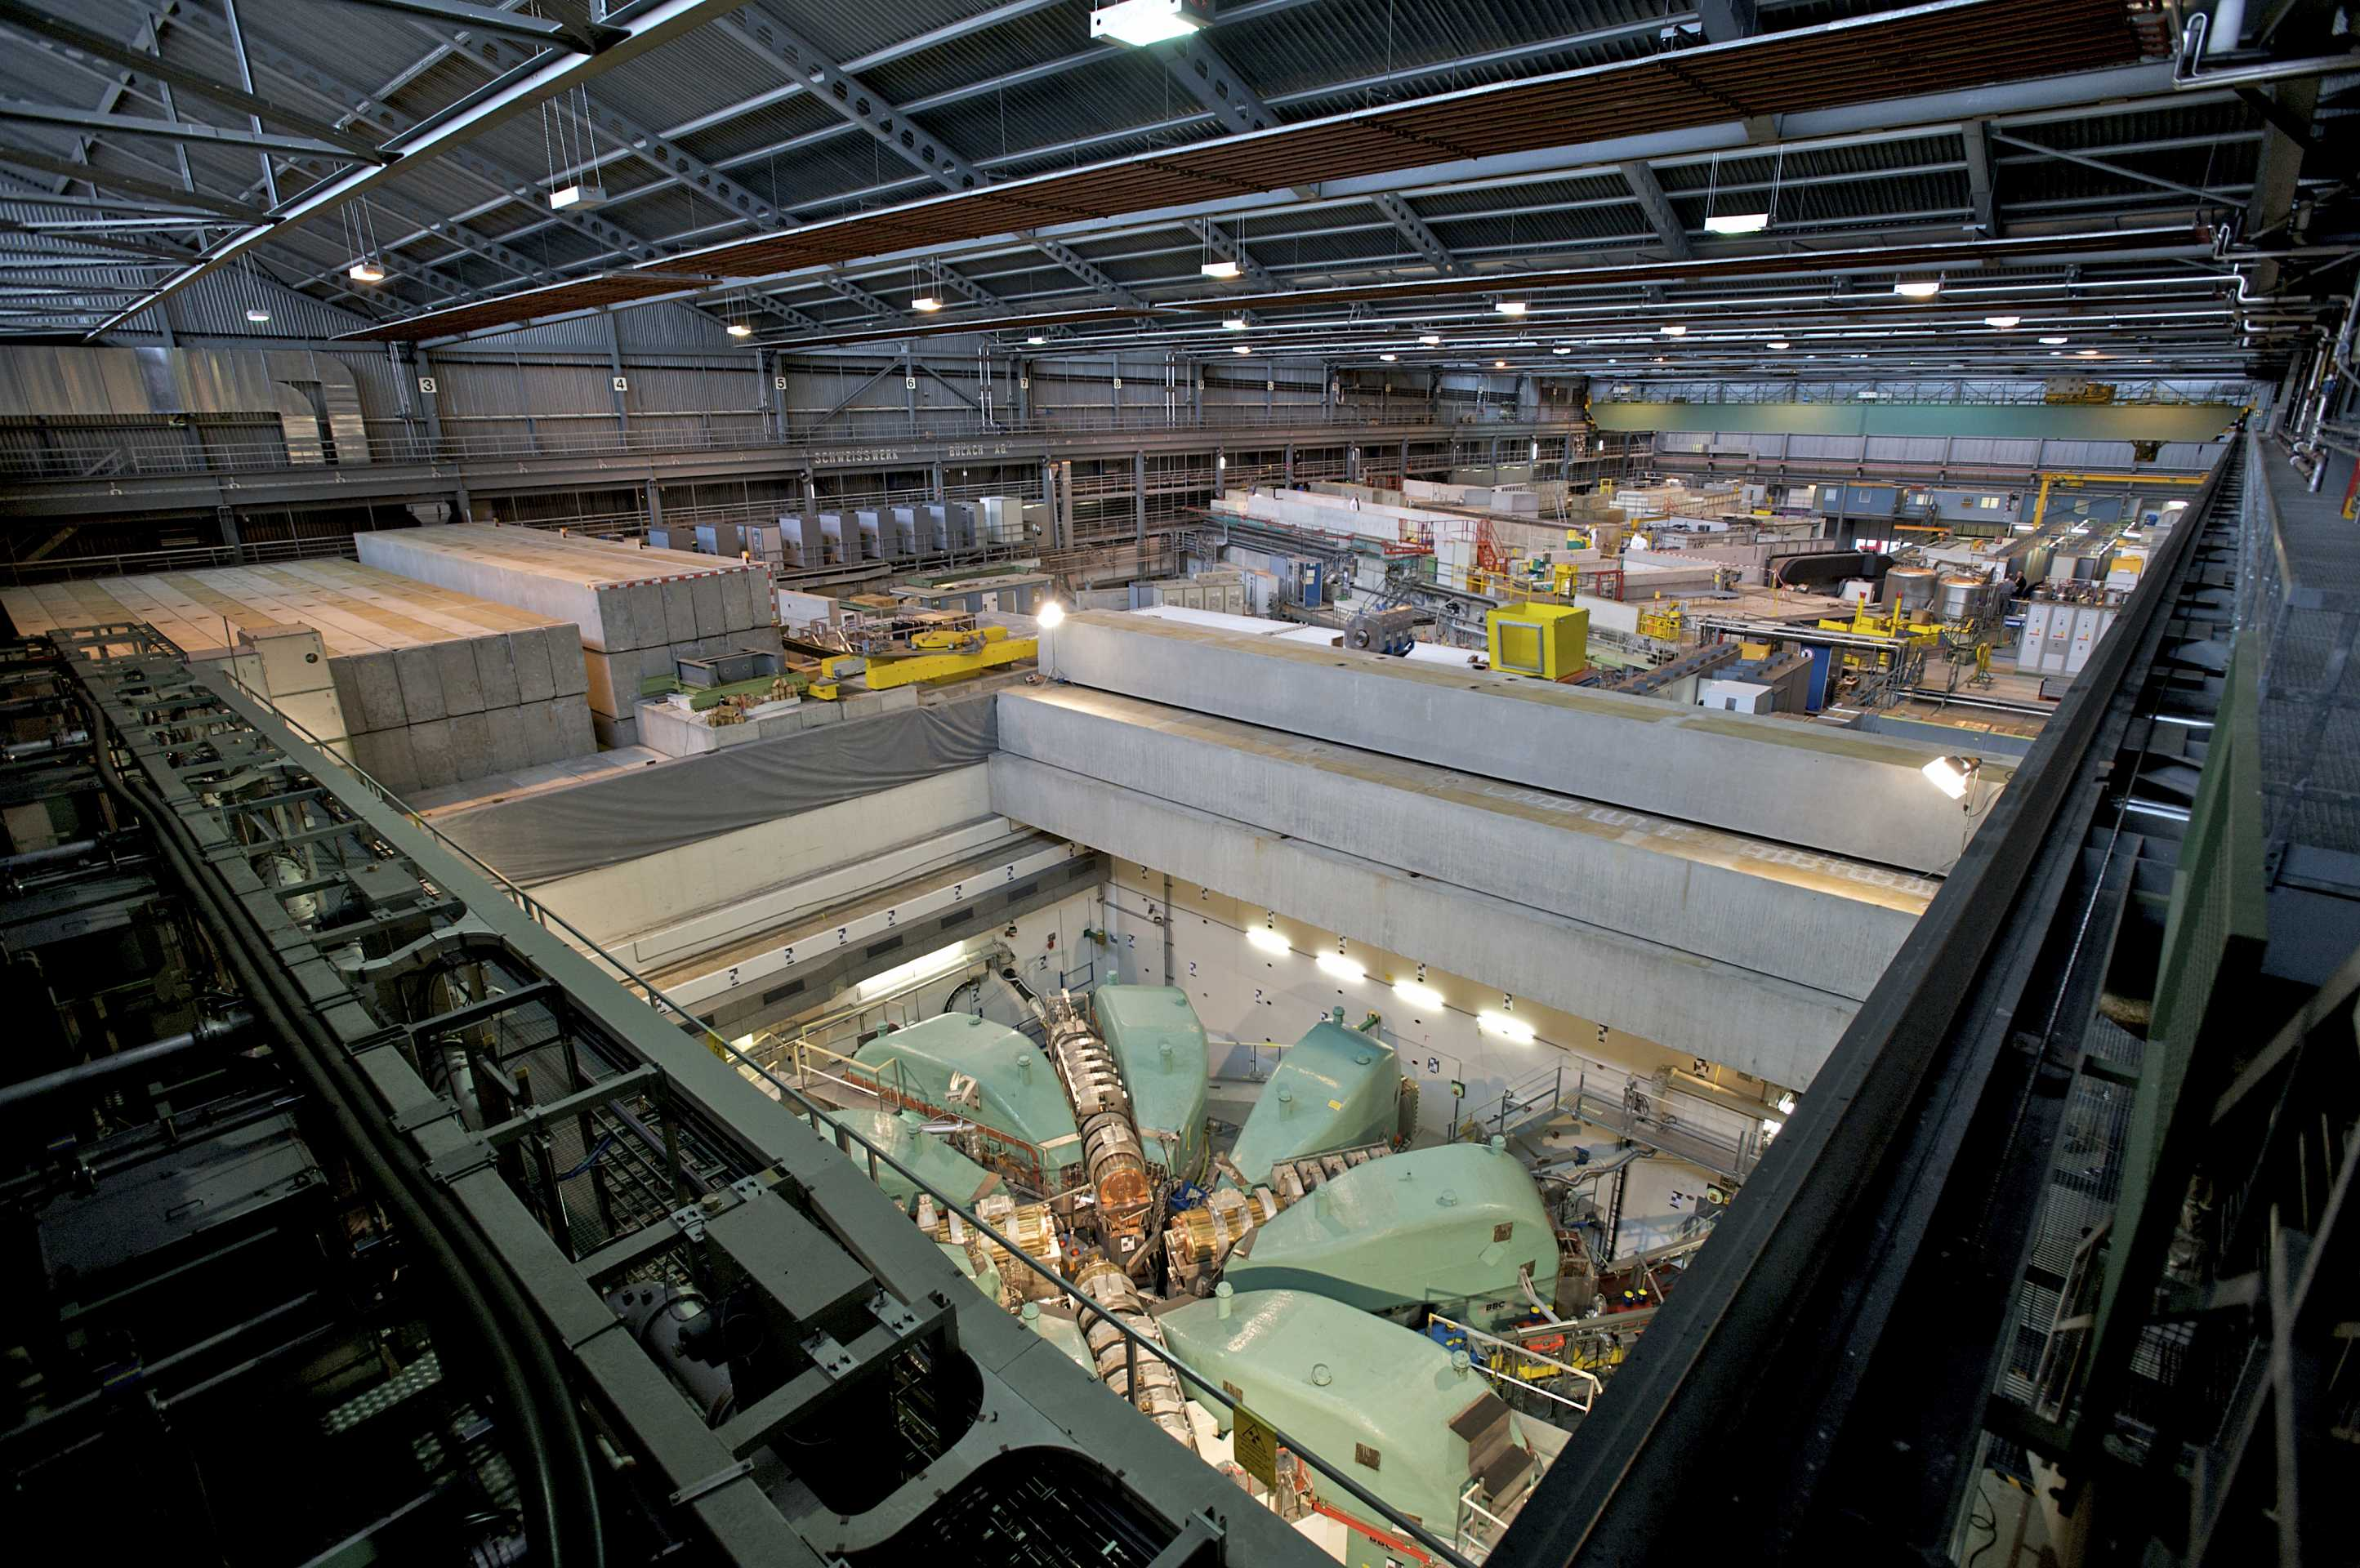
\includegraphics[width=1.15\paperwidth]{Cyclo2}};
	\end{tikzpicture}
	
\end{frame}
%%%%%%%%%%%%%%%%%%%%%%%% FRAME 1 %%%%%%%%%%%%%%%%%%%%%%%%%%%%%%%
\begin{frame}{Test Site}

	\begin{itemize}
		\itemfill
		\item High Intensity Proton Accelerator (HIPA) at PSI 
		\item beam line PiM1
		\item positive pions ($\uppi^+$) with momentum of \SI{260}{\mega\electronvolt\per c} 
		\item tunable particle fluxes from \orderof{\SI{1}{\kilo\hertz\per cm^2}} to \orderof{\SI{10}{\mega\hertz\per cm^2}}
	\end{itemize}
	
	\begin{figure}
		\centering
		\subfiga[.45]{Cyclo1}{.5}
		\subfiga[.3]{Cyclo3}{.5}
		\subfiga[.22]{Target}{.25}
	\end{figure}\vspace*{-10pt}

\end{frame}
%%%%%%%%%%%%%%%%%%%%%%%% FRAME 2 %%%%%%%%%%%%%%%%%%%%%%%%%%%%%%%
\begin{frame}{Setup}

	\begin{figure}\vspace*{-10pt}
		\centering
		\animategraphics[loop,width=.5\textwidth]{40}{t}{13}{0}
		\caption{Modular Beam Telescope}
	\end{figure}

	\begin{itemize}\itemfill
		\item 4 tracking planes \ra trigger (fast-OR) with adjustable effective area
		\item diamond pad detectors in between tracking planes
		\item low time precision of fast-OR trigger
		\item fast scintillator for precise trigger timing \ra \orderof{\SI{1}{\nano\second}}
	\end{itemize}

\end{frame}
%%%%%%%%%%%%%%%%%%%%%%%% FRAME 3 %%%%%%%%%%%%%%%%%%%%%%%%%%%%%%%
\begin{frame}{Schematic Setup}
 
	\vspace*{-10pt}\fig{SchematicsV2}{.7}
 
	\begin{itemize}\itemfill
		\item PSI DRS4 Evaluation Board as digitiser for the pad waveforms
% 		\item Digital Test Board (DTB) and pXar software for the telescope readout
		\item global trigger: coincidence of two telescope planes closest to DUTs and scintillator
	\end{itemize}

\end{frame}
%%%%%%%%%%%%%%%%%%%%%%%% FRAME 4 %%%%%%%%%%%%%%%%%%%%%%%%%%%%%%%
\begin{frame}{Pad Detectors}

	\begin{figure} 
		\centering
		\subfiga{PadBox}{.5}
		\subfiga{PadFull}{.5}
	\end{figure}\vspace*{5pt}
	
	\begin{itemize} \itemfill
		\item building the detector: cleaning, photo-lithography and Cr-Au metallisation
		\item gluing to PCBs in custom built amplifier boxes
		\item connecting to low gain, fast amplifier with \orderof{\SI{5}{\nano\second}} rise time
	\end{itemize}
	
\end{frame}

% ============= 3 =============
\section{Analysis}
%%%%%%%%%%%%%%%%%%%%%%%% FRAME 0 %%%%%%%%%%%%%%%%%%%%%%%%%%%%%%%
\begin{frame}{Waveforms}

	\vspace*{-20pt}
	\figp{SignalWaveform}{.3}\vspace*{-20pt}
	\fig{SignalWaveforms30000}{.3}\vspace*{-10pt}

	\begin{itemize}\itemfill
		\item most frequent peak (\SI{\sim70}{ns}): signal from triggered particle
		\item other peaks originate from particle of other bunches 
		\item resolve bunch spacing of PSI beam: \SI{\sim19.8}{ns}
		\item signals in in pre-signal bunch forbidden \ra noise extraction
	\end{itemize}
	
\end{frame}
%%%%%%%%%%%%%%%%%%%%%%%% FRAME 1 %%%%%%%%%%%%%%%%%%%%%%%%%%%%%%%
\begin{frame}{Signal Definition \& Calculation}
 
	\vspace*{-10pt}
	\figp{intpeaks}{.44}
	
	\begin{itemize} \itemfill
		\item define signal region: \SI{\sim\pm10}{\nano\second} around peak of the triggered signal \ra [\SI{60}{\nano\second}, \SI{80}{\nano\second}]
		\item signal: finding the peak in the signal region and integrate around it [\SI{-4}{\nano\second}, \SI{6}{\nano\second}]
		\item pedestal: integrate with same lenght (\SI{10}{\nano\second}) in the centre of the pre-trigger bunch [\SI{40}{\nano\second}, \SI{60}{\nano\second}]
% 		\item signal forbidden in pre-trigger bunch due to trigger logic
% 		\item correct for the DRS4 circular buffer length to get the length of the integral right
	\end{itemize}
 
\end{frame}
%%%%%%%%%%%%%%%%%%%%%%%% FRAME 2 %%%%%%%%%%%%%%%%%%%%%%%%%%%%%%%
\begin{frame}{Signal To Noise Ratio}
	
	\begin{figure}\vspace*{-15pt}
		\centering
		\subfigpa{SNR1}{.5}
		\subfigpa{SNR2}{.5}
	\end{figure}
% 	\begin{center} \missingfigure[figheight=.5\textheight,figwidth=.5\textheight , figcolor=white]{}\end{center}
	
	\begin{itemize}\itemfill
		\item optimise SNR by scanning the integral width in both directions
		\item flat plateau around the the FWHM of the waveform peak
	\end{itemize}
 
\end{frame}


% ============= 4 =============
\section{Results}
%%%%%%%%%%%%%%%%%%%%%%%% FRAME 0 %%%%%%%%%%%%%%%%%%%%%%%%%%%%%%%
\begin{frame}{Noise Distributions at \SI{\sim10}{\mega\hertz\per\centi\meter^2}}
 
	\begin{figure}\vspace*{-15pt}
		\centering
		\subfigp{PD0}{.5}{scCVD with \SI{6}{\deci\bel} attenuation}
		\subfigp{PD1}{.5}{pCVD}
	\end{figure}\vspace*{-10pt}

	\begin{itemize} \itemfill
		\item noise distribution agrees well with Gaussian even at high rates
		\item extract noise by taking the sigma of the Gaussian fit
		\item noise similar for scCVD and pCVD diamond
	\end{itemize}
 
\end{frame}
%%%%%%%%%%%%%%%%%%%%%%%% FRAME 1 %%%%%%%%%%%%%%%%%%%%%%%%%%%%%%%
\begin{frame}{Signal Distributions at \SI{\sim10}{\mega\hertz\per\centi\meter^2}}
 
	\begin{figure}\vspace*{-15pt}
		\centering
		\subfigp{SD0}{.5}{scCVD with \SI{6}{\deci\bel} attenuation}
		\subfigp{SD1}{.5}{pCVD}
	\end{figure}\vspace*{-10pt}

	\begin{itemize} \itemfill
		\item signal gets corrected by the mean of the noise (baseline offset)
		\item pCVD signal smaller and smeared by different regions in the diamond
	\end{itemize}
 
\end{frame}
%%%%%%%%%%%%%%%%%%%%%%%% FRAME 2 %%%%%%%%%%%%%%%%%%%%%%%%%%%%%%%
\begin{frame}{Signal Maps}
 
	\begin{figure}\vspace*{-15pt}
		\centering
		\subfigp{SM0}{.5}{scCVD with \SI{6}{\deci\bel} attenuation}
		\subfigp{SM1}{.5}{pCVD}
	\end{figure}
	
	\begin{itemize} \itemfill
		\item flat signal distribution in scCVD
		\item signal response depending on region in the pCVD
	\end{itemize}
 
\end{frame}
%%%%%%%%%%%%%%%%%%%%%%%% FRAME 3 %%%%%%%%%%%%%%%%%%%%%%%%%%%%%%%
\begin{frame}{Currents}
 
	\vspace*{-15pt}\fig{Currents.png}{.6}
	
	\begin{itemize} \itemfill
		\item typical rate scans for \SI{\sim30}{\hour} with rates up to \SI{\sim20}{\mega\hertz\per\centi\meter^2}
		\item beam induced current clearly visible
		\item low leakage currents (\SI{<30}{\nano\ampere}) at a bias voltage of \SI{-1000}{\volt} (\SI{2}{\volt\per\micro m})
	\end{itemize}
 
\end{frame}
%%%%%%%%%%%%%%%%%%%%%%%% FRAME 4 %%%%%%%%%%%%%%%%%%%%%%%%%%%%%%%
\begin{frame}{Rate Studies}

	
	\vspace*{-15pt}
	\figp{B2Oct15}{.65} 
	
	\begin{itemize}
		\item systematically checking several up and down scans
		\item also random scans to rule out systematic effects 
	\end{itemize}
	
\end{frame}
%%%%%%%%%%%%%%%%%%%%%%%% FRAME 5 %%%%%%%%%%%%%%%%%%%%%%%%%%%%%%%
\begin{frame}{Rate Studies in Non-Irradiated scCVD}

	
	\vspace*{-15pt}
	\figp{S129Scans}{.65} 
	
	\begin{itemize}
		\item scCVD as reference in all beam tests
		\item all scans scaled to 1 and shifted for display
		\item scCVD diamond shows now rate dependence within the measurement precision
	\end{itemize}
	
\end{frame}
%%%%%%%%%%%%%%%%%%%%%%%% FRAME 6 %%%%%%%%%%%%%%%%%%%%%%%%%%%%%%%
\begin{frame}{Rate Studies in Irradiated pCVD}

	\vspace*{-15pt}
	\figp{B2Scans}{.65}
	
	\begin{itemize}
		\itemfill
		\item all scans scaled to 1 and shifted for display
		\item pulse height very stable after irradiation
		\item noise stays the same of: $\upsigma \approx$ \SI{4.9}{au}
% 		\item signal degradation due to radiation damage (no absolute calibration)
	\end{itemize}

\end{frame}

% ============= CONCLUSION =============
\section{Conclusion}
\begin{frame}{Conclusion}

	\begin{minipage}[c][.5\textheight]{\textwidth}
		\begin{itemize}
			\itemfill
			\item built beam test setup to characterise the rate behaviour of diamond pad detectors
			\item pCVD diamond show different signal response depending on the position in the diamond
			\item nonirradiated scCVD show no rate dependence
			\item detectors with irradiated pCVD diamond sensors can be built which have a rate dependence below \SI{2}{\%} up to a flux of \SI{20}{\mega\hertz\per \centi\meter^2}
		\end{itemize}
	\end{minipage}
	
\end{frame}


% ============= ACKNOWLEDGEMENTS =============
{\usebackgroundtemplate{\tikz\node[opacity=0.2] {\hspace*{-5pt}
\includegraphics[height=\paperheight,width=1.05\paperwidth]{back.jpg}};}
\begin{frame}{Acknowledgements}

	\begin{center}
		\ETHlogo[5cm]
	\end{center}\vspace*{20pt}
	
	\begin{figure}
		\centering
		\subfiga{ohio-logo}{.3}
		\subfiga{psi-logo}{.2}
	\end{figure}\vspace*{20pt}
	
	\begin{center}
		\begin{Huge}\textbf{The RD42 Collaboration}\end{Huge}
	\end{center}

	
\end{frame}}


\begin{frame}{Acknowledgements}

	\begin{tikzpicture}[remember picture,overlay]
		\node[at=(current page.center)] {
			
\includegraphics[width=1.12\paperwidth]{delfin}};
	\end{tikzpicture}
	
\end{frame}


% DOCUMENT END
\end{document}

